\documentclass[oneside,openright,12pt]{ufsm_2021} 

\include{dados/dados}
\include{dados/opcoes-formatacao}

\include{pre-textuais/ficha-catalografica}
\dedicatoria{Dedico este trabalho a todos que são apaixonados por computação.}
\agradecimentos{
    Agradeço primeiramente a Deus por ter me dado as oportunidades que tive e por me manter firme durante todo o processo de desenvolvimento deste trabalho.

    Agradeço aos meus pais, Joacir Felix da Trindade e Sirlei Souza Costa, por todo suporte e por sempre acreditarem em mim. 

    Agradeço à minha família e aos amigos pelo apoio e pela motivação que me ajudaram durante a produção deste trabalho.    
    
    Agradeço à Universidade Federal de Santa Maria (UFSM) e a todos os professores do curso de Sistemas para Internet com os quais tive contato durante a graduação, que mantiveram viva a minha paixão pelo conhecimento e me tornaram não apenas um profissional, mas uma pessoa melhor.
    
    Agradeço à empresa Conplan Sistemas por permitir que eu fizesse horários flexíveis para assistir às aulas e ir às reuniões de orientação necessárias para a conclusão deste trabalho.
    
    Ao Pr. Vanderlei Jesus de Andrade dos Reis e à sua família, expresso minha gratidão pelo acolhimento e apoio desde a minha chegada à cidade de Santa Maria.

    Ao meu orientador, Professor Dr. Leandro Oliveira Freitas, agradeço pelos direcionamentos e pela dedicação ao longo dessa jornada. Estendo meus agradecimentos aos membros da banca avaliadora pela disponibilidade e pelo aceite em analisar meu trabalho.
}
\epigrafe{``The people who are crazy enough to think they can change the world are the ones who do.''}{Apple, ``Think Different'' Campaign (1997)} 
\include{pre-textuais/resumo}


% % %  ATIVACAO DE LISTAS E PAGINAS ESPECIAIS
% % %  PARA QUE APARECAO NAO NO TEXTO DESCOMENTE A LINHA ABAIXO -> POR PADRAO TODAS ESTAO ATIVIDADAS

% % LISTA DE FIGURAS 
% \semfiguras   %%(QUANDO ATIVIDA NAO EXIBE A LISTA)

% % LISTA DE GRAFICOS 
\semgraficos   %%(QUANDO ATIVIDA NAO EXIBE A LISTA)

% % LISTA DE ILUSTRACOES 
\semilustracoes  %%(QUANDO ATIVIDA NAO EXIBE A LISTA)

% % LISTA DE TABELAS 
\semtabelas   %%(QUANDO ATIVIDA NAO EXIBE A LISTA)

% % LISTA DE QUADROS 
%\semquadros   %%(QUANDO ATIVIDA NAO EXIBE A LISTA)

% % LISTA DE APENDICES 
\semapendices  %%(QUANDO ATIVIDA NAO EXIBE A LISTA)

% LISTA DE ANEXOS 
\semanexos   %%(QUANDO ATIVIDA NAO EXIBE A LISTA)


% % % %  LISTA DE ABREVIATURAS - AMBIENTE TABULAR
%%%%%%%% para não utilizar comente as linhas abaixo.
\abreviaturamax{SIGLAMAX} %%%% coloque aqui a maior sigla (indentacao)
\listadeabreviaturas{
    MVC & Model-View-Controller \\
    SRP & Single Responsibility Principle \\
    OCP & Open/Closed Principle  \\
    LSP & Liskov Substitution Principle \\
    ISP & Interface Segregation Principle \\
    DIP & Dependency Inversion Principle \\
    BD & Banco de Dados \\
    UI & User Interface \\
    HTTP & Hypertext Transfer Protocol \\
    JSON & JavaScript Object Notation \\
    ORM & Object-Relational Mapping \\ 
    REST & Representational State Transfer \\
    CGI & Common Gateway Interface \\ 
    PET & Programa de Educação Tutorial
}


% % % %  LISTA DE SIGLAS - AMBIENTE TABULAR
%%%%%%%% para não utilizar comente as linhas abaixo.
%%\siglamax{SIGLAMAX} %%%% coloque aqui a maior sigla (indentacao)
%%\listadesiglas{
%%SIGLA1 & Nome Completo da Sigla 1 \\
%%SIGLA2 & Nome Completo da Sigla 2 \\
%%SIGLAMAX &	Nome Completo da Sigla MAX \\
%%}


% % % %  LISTA DE SIMBOLOS
%%%%%%%% OBS: O espaco entre colchetes \item[] e um ambiente matematico
%%%%%%%% para não utilizar comente as linhas abaixo.
%%\simbolomax{(Re)2} %%%% coloque aqui o maior simbolo (indentacao)
%%\listadesimbolos{
%%\item[u_*]	Escala de velocidade de fricção	
%%\item[w_*]	Escala de velocidade convectiva
%%\item[(Re)^2]	Maior simbolo da lista
%%}

%% \include{pre-textuais/folha-de-errata}

% PACOTES
\usepackage{booktabs}
\usepackage{tabularx}
\usepackage{caption}
\usepackage{graphicx} 
\usepackage{float} 
\usepackage{svg}
\usepackage{tikz}
\usepackage{listings}
\usepackage{xcolor}
\usepackage{dirtree}

% CONFIGURACAO DA LISTA DE CODIGOS
\renewcommand{\lstlistingname}{Código}
\renewcommand{\lstlistlistingname}{Lista de Códigos}

\definecolor{phpkeyword}{RGB}{0,0,180}   % azul escuro
\definecolor{phpcomment}{RGB}{0,128,0}   % verde
\definecolor{phpstring}{RGB}{180,0,0}    % vermelho

\captionsetup[lstlisting]{
    font=footnotesize
}
\lstset{
    language=PHP,                          % linguagem PHP
    basicstyle=\ttfamily\scriptsize\setstretch{1},
    keywordstyle=\color{phpkeyword}\bfseries, % palavras-chave em azul e negrito
    commentstyle=\color{phpcomment},       % comentários em verde
    stringstyle=\color{phpstring},         % strings em vermelho
    numbers=left,                          % números das linhas à esquerda
    numberstyle=\tiny\color{gray},         % estilo dos números
    stepnumber=1,                          % mostra número a cada linha
    showstringspaces=false,                % não mostrar espaços em strings
    breaklines=true,                       % quebra automática de linha
    frame=single,                          % quadro ao redor do código
    tabsize=4,                             
    escapeinside={(*@}{@*)},               % escape para LaTeX dentro do código
    morekeywords={private,public,protected,final,interface,implements,extends},
    captionpos=t,
    aboveskip=18pt,  
    belowskip=18pt
}

% DOCUMENTO
\begin{document}
    \pretextual
    
    %% TEXTUAIS
    \include{textuais/introducao}
    \chapter{Levantamento bibliográfico}
    \section{Introdução ao capítulo}
        \par Este capítulo tem como objetivo apresentar os conceitos de MVC e Arquitetura Limpa, usando dos estudos dos autores aqui citados para promover uma base teórica sólida para o entendimento das implementações futuras feitas nesse trabalho, bem como as análises da literatura.
    
    \input{textuais/levantamento_bibliografico/1.padrao_mvc}
    \input{textuais/levantamento_bibliografico/2.arquitetura_limpa}
    \subsection{Princípios SOLID}

    \par Os princípios SOLID, um acrônimo popularizado por Michael Feathers com base nos trabalhos de Robert C. Martin, representam cinco diretrizes cruciais para o design de software orientado a objetos. Estes princípios foram concebidos para auxiliar os desenvolvedores a construir sistemas que sejam mais fáceis de entender, manter e evoluir, aplicando-se a classes em qualquer camada da aplicação para se alcançar um melhor design, o que, por sua vez, contribui para uma base de código flexível e de fácil manutenção \cite{livro:joshi:2016}.

    \par A adesão a estes cinco preceitos — Princípio da Responsabilidade Única (SRP), Princípio Aberto/Fechado (OCP), Princípio da Substituição de Liskov (LSP), Princípio da Segregação de Interface (ISP) e Princípio da Inversão de Dependência (DIP) — é fundamental para o desenvolvimento de software de alta qualidade. Eles oferecem um vocabulário comum e um conjunto de heurísticas para a discussão e avaliação da arquitetura de software, direcionando as práticas de desenvolvimento para a minimização de dependências e o aprimoramento da coesão do código \cite{artigo:ramachandrappa:2024}.
    
    \par Cada princípio é descrito abaixo, com sua aplicação e exemplos práticos.

%
%
% SRP
%
%
    
\subsection{Princípio da Responsabilidade Única (Single Responsibility Principle - SRP)}
    
    \par O Princípio da Responsabilidade Única (SRP) preconiza que um módulo, ou mais comumente uma classe, deve ter uma, e apenas uma, razão para mudar, o que implica ser responsável por um único ator ou aspecto da funcionalidade do sistema. Este princípio está intimamente ligado ao conceito de coesão, onde um módulo coeso agrupa funcionalidades que servem a um único propósito bem definido. O objetivo é garantir que cada classe realize uma tarefa específica, simplificando sua compreensão e manutenção \cite{livro:martin:cleanarch}.

    \par A aplicação do SRP é vital, pois assegura que cada classe permaneça dedicada a uma tarefa específica, o que, por sua vez, simplifica seu entendimento, manutenção e potencial de expansão. Quando as classes seguem o SRP, elas se tornam mais diretas para refatorar, testar e estender, e modificações são menos propensas a afetar outras partes do sistema, minimizando o risco de introduzir erros. Isso é um contraste com classes que acumulam múltiplas responsabilidades, as quais se tornam complexas e frágeis \cite{artigo:ramachandrappa:2024}.

    \par Segue um exemplo prático de violação do SRP, conforme pode ser visualizado na Figura~\ref{fig:figura_srp_bad} que demonstra a situação ANTES da aplicação do princípio:
        
    \begin{figure}[H]
        \centering
        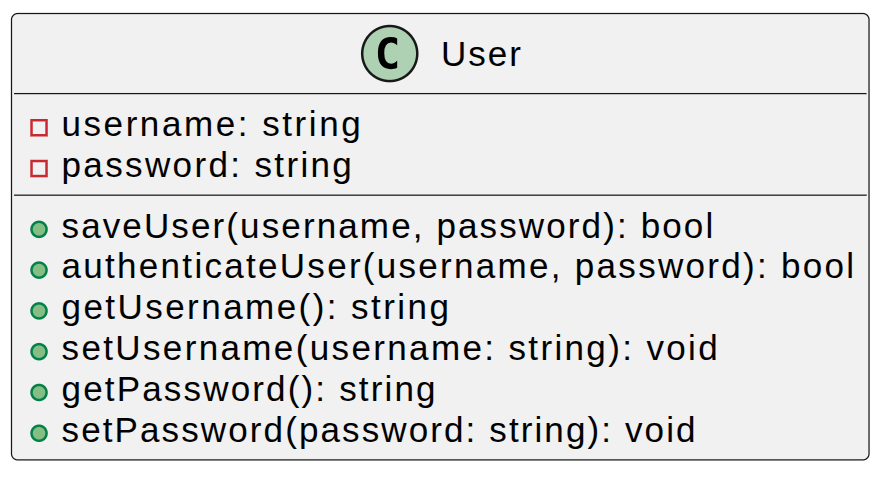
\includegraphics[width=0.8\textwidth]{figuras/solid/srp_bad.png}
        \caption{Violação do SRP.}
        \label{fig:figura_srp_bad}
        \newcommand{\minhafonte}{Fonte: Adaptado de \cite{artigo:ramachandrappa:2024}.}
        \minhafonte
    \end{figure}

    \par Nesse exemplo trazido por \cite{artigo:ramachandrappa:2024} a classe User que lida tanto com a gestão dos dados do usuário (como nome e senha) quanto com a lógica de autenticação desse usuário, como no método AuthenticateUser. 
    
    \par A Figura~\ref{fig:figura_srp_good} ilustra a situação DEPOIS da refatoração para fazer uso do SRP:

    \begin{figure}[H]
        \centering
        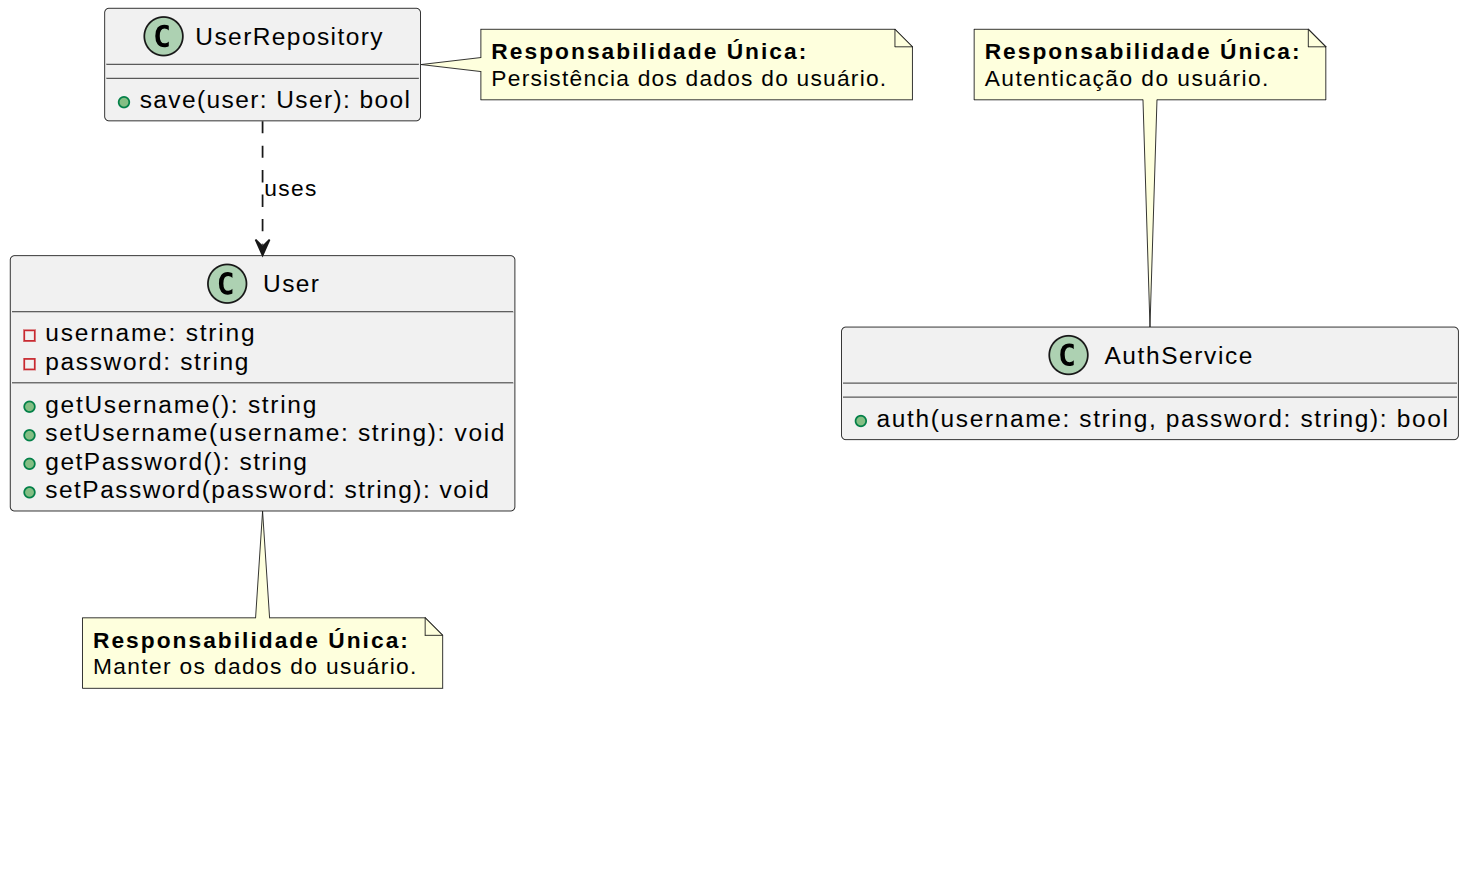
\includegraphics[width=0.9\textwidth]{figuras/solid/srp_good.png}
        \caption{Aplicação do SRP.}
        \label{fig:figura_srp_good}
        \newcommand{\minhafonte}{Fonte: Adaptado de \cite{artigo:ramachandrappa:2024}.}
        \minhafonte
    \end{figure}

    \par Na Figura~\ref{fig:figura_srp_good} a classe User mantêm apenas os dados, a classe UserRepository controla a persistência e AuthService gerenciaria a autenticação, assim demonstrando o uso da SRP, onde cada classe tem sua própria responsabilidade \cite{artigo:ramachandrappa:2024}.

        

%
%
% OPC
%
%
\subsection{Princípio Aberto/Fechado (Open/Closed Principle - OCP)}

    \par O OCP determina que classes devem ser abertas para extensão, mas fechadas para modificação, assim permitindo a adição de funcionalidades sem alterar o código existente \cite{livro:martin:cleanarch}. Na Arquitetura Limpa, o OCP é implementado por meio de interfaces e herança, especialmente em adaptadores, para suportar novas integrações \cite{livro:martin:cleanarch}. 

    \par O Princípio Aberto/Fechado (OCP), conforme articulado por Bertrand Meyer, estabelece que entidades de software, como classes, módulos ou funções, devem ser abertas para extensão, mas fechadas para modificação. Isso significa que o comportamento de um sistema deve poder ser estendido através da adição de novo código, em vez de alterar código existente que já foi testado e está em funcionamento. Este princípio visa proteger o código existente de regressões e reduzir a necessidade de retestes extensivos \cite{livro:martin:cleanarch}.

    \par Seguir o OCP é crucial para manter a estabilidade do software à medida que ele evolui, permitindo que novas funcionalidades sejam integradas sem comprometer as existentes. Ao aderir ao OCP, os desenvolvedores podem adicionar novas funcionalidades sem alterar o código base existente, o que minimiza o risco de introduzir novos bugs. Este princípio é crucial para criar sistemas que podem crescer e se adaptar ao longo do tempo com menor esforço de manutenção \cite{artigo:ramachandrappa:2024}.


    \par Considere uma classe DiscountCalculator que calcula descontos com base em diferentes tipos de cliente através de múltiplas declarações if-else if, como pode ser visualizado no diagrama ANTES da aplicação do OCP:

     \begin{figure}[H]
        \centering
        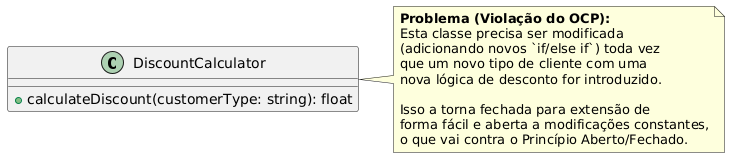
\includegraphics[width=0.8\textwidth]{figuras/solid/ocp_bad.png}
        \caption{Violação da OCP.}
        \label{fig:figura_ocp_bad}
        \newcommand{\minhafonte}{Fonte: Adaptado de \cite{artigo:ramachandrappa:2024}.}
        \minhafonte
    \end{figure}
        
    Para aplicar o OCP, como demonstrado no diagrama DEPOIS da aplicação do OCP:

     \begin{figure}[H]
        \centering
        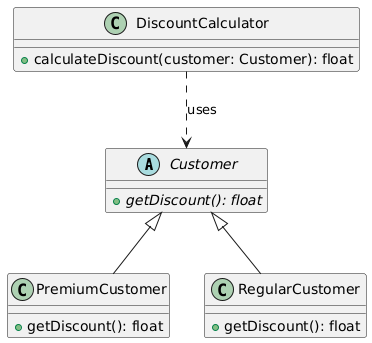
\includegraphics[width=0.5\textwidth]{figuras/solid/ocp_good.png}
        \caption{Aplicação da OCP.}
        \label{fig:figura_ocp_good}
        \newcommand{\minhafonte}{Fonte: Adaptado de \cite{artigo:ramachandrappa:2024}.}
        \minhafonte
    \end{figure}

    pode-se usar polimorfismo: uma classe abstrata Customer com um método abstrato GetDiscount(). As classes RegularCustomer e PremiumCustomer herdariam de Customer e implementariam GetDiscount(). Assim, o DiscountCalculator usaria o método GetDiscount() do objeto Customer passado, permitindo a adição de novos tipos de clientes criando novas subclasses de Customer sem alterar o DiscountCalculator \cite{artigo:ramachandrappa:2024}.



%
%
% LSP
%
%
\subsection{Princípio da Substituição de Liskov (Liskov Substitution Principle - LSP)}

    \par O Princípio da Substituição de Liskov (LSP), formulado por Barbara Liskov, dita que instâncias de uma classe pai devem ser substituíveis por instâncias de uma classe derivada sem alterar a corretude ou o comportamento esperado do programa. Este princípio é crucial para guiar o uso da herança de forma a manter a integridade e a previsibilidade do sistema. Essencialmente, uma subclasse deve poder ser utilizada em qualquer lugar onde sua superclasse é esperada, sem causar efeitos colaterais indesejados \cite{livro:martin:cleanarch}.

    \par Aderir ao LSP é fundamental para o uso correto do polimorfismo e da herança, resultando em código mais confiável e de fácil manutenção, especialmente em sistemas grandes onde o polimorfismo é intensamente utilizado. Quando o LSP é respeitado, as hierarquias de classes são mais robustas, e a capacidade de substituição garante que o sistema se comporte de maneira consistente, independentemente da implementação específica da subclasse utilizada \cite{livro:joshi:2016}.
    
    \par Um exemplo clássico de violação do LSP, que pode ser detalhado no diagrama ANTES da aplicação do LSP:
    
    \begin{figure}[H]
        \centering
        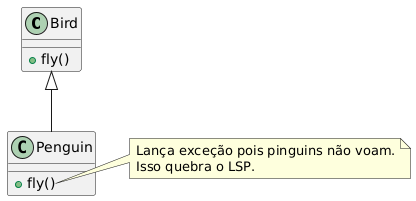
\includegraphics[width=0.7\textwidth]{figuras/solid/lsp_bad.png}
        \caption{Violação da LSP.}
        \label{fig:solid/lsp_bad}
        \newcommand{\minhafonte}{Fonte: Adaptado de \cite{artigo:ramachandrappa:2024}.}
        \minhafonte
    \end{figure}
    
    ocorre com as classes Rectangle e Square, ou Bird e Penguin. No caso Bird/Penguin, se Penguin herda de Bird e o método Fly() em Bird implica a capacidade de voar, a implementação de Fly() em Penguin (que não voa) lançando uma exceção violaria o LSP. Uma solução, apresentada no diagrama DEPOIS da refatoração:
    
    \begin{figure}[H]
        \centering
        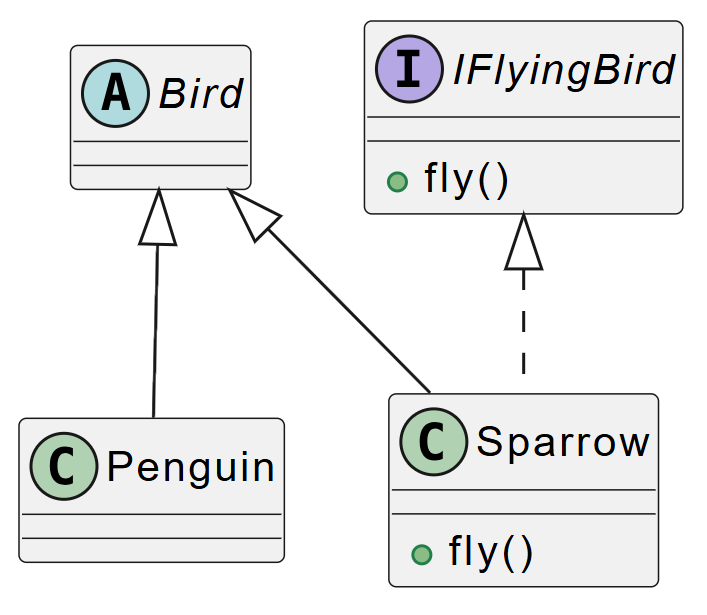
\includegraphics[width=0.5\textwidth]{figuras/solid/lsp_good.png}
        \caption{Aplicação da LSP.}
        \label{fig:figura_lsp_good}
        \newcommand{\minhafonte}{Fonte: Adaptado de \cite{artigo:ramachandrappa:2024}.}
        \minhafonte
    \end{figure}
    
    poderia envolver hierarquias mais adequadas ou interfaces específicas para as capacidades, como uma interface IFlyingBird não implementada por Penguin \cite{artigo:ramachandrappa:2024}.


%
%
% ISP
%
%
\subsection{Princípio da Segregação de Interface (Interface Segregation Principle - ISP)}
    
    \par O Princípio da Segregação de Interface (ISP) orienta que os clientes de uma classe não devem ser forçados a depender de métodos que não utilizam. Este princípio promove a criação de interfaces menores, coesas e específicas para as necessidades de cada cliente, em detrimento de interfaces grandes e genéricas que tentam abranger múltiplas funcionalidades. O objetivo é evitar que classes implementem métodos desnecessários, o que pode levar a um acoplamento indesejado \cite{livro:martin:cleanarch}.

    \par A aplicação do ISP é importante para promover o desacoplamento, assegurando que as classes dependam apenas das interfaces que são estritamente relevantes para elas. Isso não apenas reduz o impacto de futuras alterações – já que uma mudança em uma interface específica afeta apenas os clientes que a utilizam – mas também torna a base de código mais flexível, modular e fácil de testar. Interfaces menores são mais fáceis de entender e implementar corretamente \cite{artigo:ramachandrappa:2024}.
    
    \par Um exemplo de violação do ISP, que pode ser visualizado na Figura~\ref{fig:figura_isp_bad}:
    
     \begin{figure}[H]
        \centering
        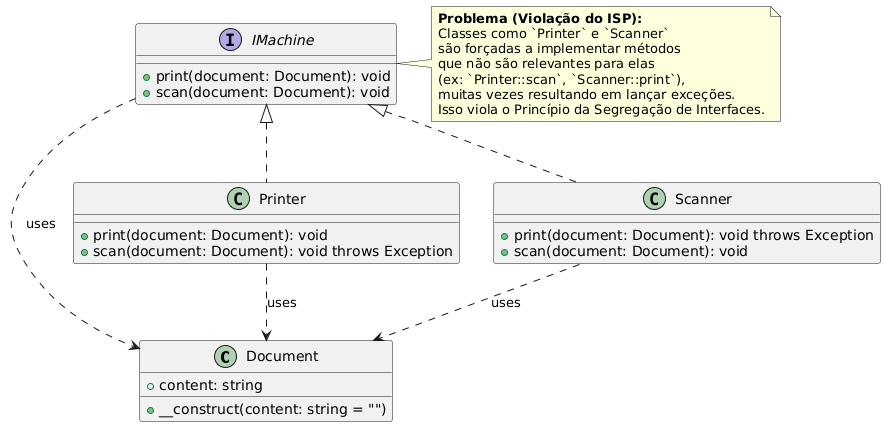
\includegraphics[width=0.9\textwidth]{figuras/solid/isp_bad.png}
        \caption{Violação da ISP.}
        \label{fig:figura_isp_bad}
        \newcommand{\minhafonte}{Fonte: Adaptado de \cite{artigo:ramachandrappa:2024}.}
        \minhafonte
    \end{figure}
    
    é uma interface IMachine que declara métodos como Print(Document document) e Scan(Document document). Uma classe Printer que implementa IMachine seria forçada a implementar Scan(). Para aderir ao ISP, como mostrado no diagrama das interfaces segregadas:
    
    \begin{figure}[H]
        \centering
        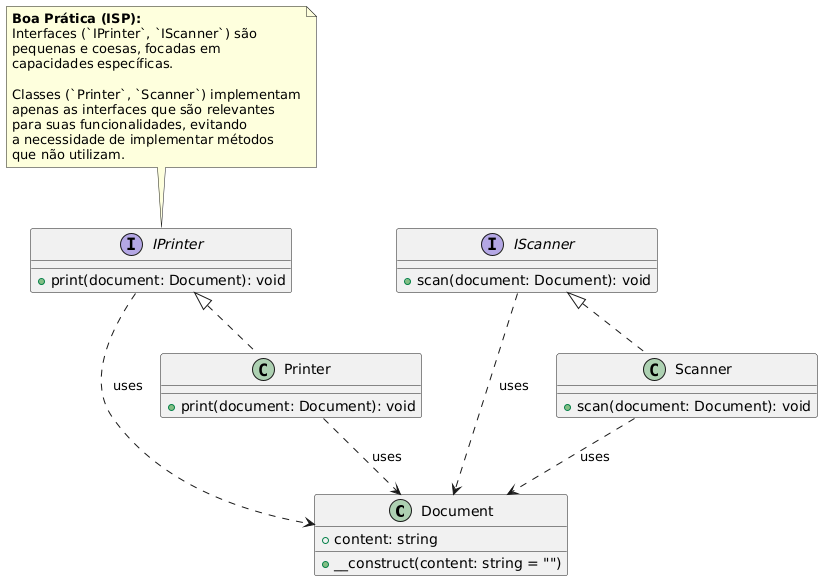
\includegraphics[width=0.9\textwidth]{figuras/solid/isp_good.png}
        \caption{Aplicação da ISP.}
        \label{fig:figura_isp_good}
        \newcommand{\minhafonte}{Fonte: Adaptado de \cite{artigo:ramachandrappa:2024}.}
        \minhafonte
    \end{figure}
    
    IMachine seria dividida em interfaces mais granulares, como IPrinter e IScanner, permitindo que Printer implemente apenas IPrinter \cite{artigo:ramachandrappa:2024}.
        
\subsection{Princípio da Inversão de Dependência (Dependency Inversion Principle - DIP)}
    
    \par O Princípio da Inversão de Dependência (DIP) estabelece que módulos de alto nível não devem depender de módulos de baixo nível; ambos devem depender de abstrações. Adicionalmente, as abstrações não devem depender de detalhes concretos, mas sim os detalhes é que devem depender das abstrações. Isso significa que as classes que contêm a lógica de negócios principal (alto nível) não devem ser diretamente acopladas a classes que lidam com detalhes de infraestrutura (baixo nível) \cite{livro:martin:cleanarch}.

    \par Este princípio é crucial para criar sistemas desacoplados e flexíveis, pois promove a dependência de interfaces ou classes abstratas em vez de implementações concretas. Isso permite que as implementações de baixo nível possam ser alteradas ou substituídas sem impactar os módulos de alto nível, desde que o contrato definido pela abstração seja mantido. Tal desacoplamento também facilita os testes, permitindo a substituição de dependências reais por dublês de teste \cite{livro:joshi:2016}

    Considere o exemplo no diagrama na Figura~\ref{fig:figura_dip_bad} que ilustra a dependência concreta:

    \begin{figure}[H]
        \centering
        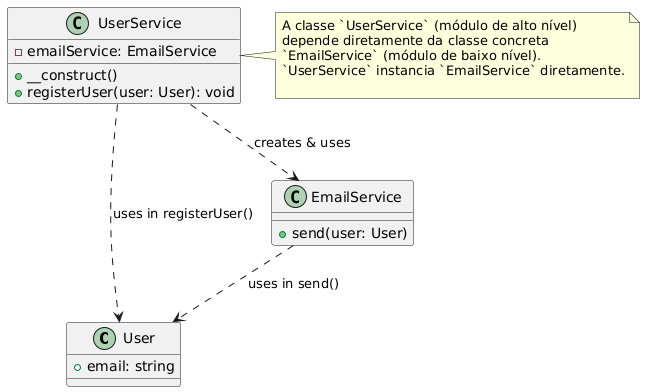
\includegraphics[width=0.9\textwidth]{figuras/solid/dip_bad.png}
        \caption{Violação da DIP.}
        \label{fig:figura_dip_bad}
        \newcommand{\minhafonte}{Fonte: Adaptado de \cite{artigo:ramachandrappa:2024}.}
        \minhafonte
    \end{figure}

    onde uma classe UserService (alto nível) que depende diretamente de uma classe concreta EmailService (baixo nível) está fortemente acoplada. Para aplicar o DIP, como ilustrado no diagrama que demonstra a inversão de dependência:

    
    \begin{figure}[H]
        \centering
        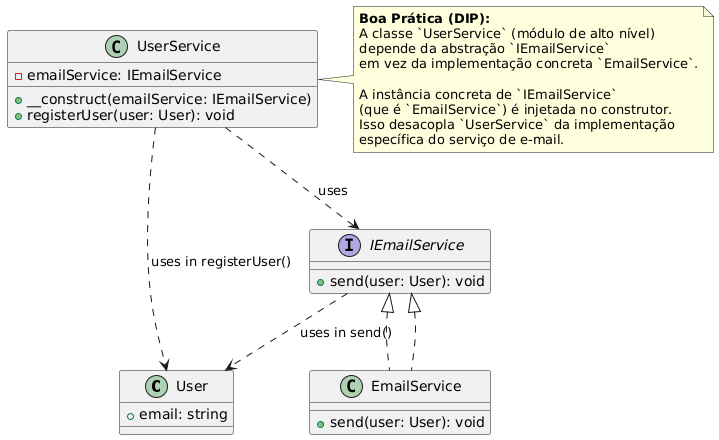
\includegraphics[width=0.9\textwidth]{figuras/solid/dip_good.png}
        \caption{Aplicação da DIP.}
        \label{fig:figura_dip_good}
        \newcommand{\minhafonte}{Fonte: Adaptado de \cite{artigo:ramachandrappa:2024}.}
        \minhafonte
    \end{figure}
    
    \par Nesse cado seria criada uma interface IEmailService. UserService dependeria de IEmailService (frequentemente via injeção de dependência), e EmailService implementaria IEmailService. Isso inverte a direção da dependência \cite{artigo:ramachandrappa:2024}.
     \subsection{Camadas da Arquitetura Limpa}
        \par A Arquitetura Limpa tem por objetivo organizar o sistema em camadas concêntricas, ou seja, com dependências apontando para dentro, conforme a Regra da Dependência. As camadas incluem entidades, casos de uso, adaptadores de interface, frameworks e drivers, conectados por limites que garantem desacoplamento \cite{livro:martin:cleanarch}.
        
        \par Abaixo segue a explicação para cada um desses conceitos, que são a base para o entendimento da arquitetura limpa.

         \begin{figure}[H] % O [H] exige o uso do pacote float (veja abaixo)
            \centering
            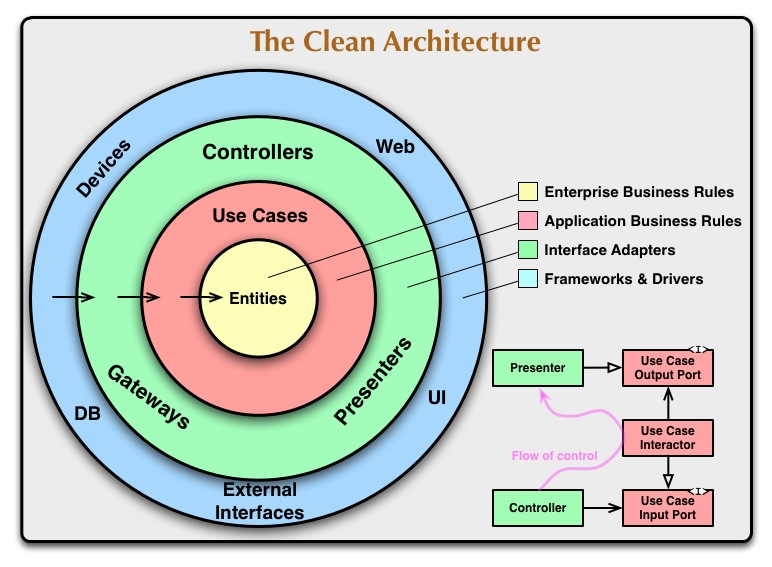
\includegraphics[width=0.8\textwidth]{figuras/clean_arch_1.jpg}
            \caption{A arquitetura limpa}
            \label{fig:figura_clean_arch_1}
            \newcommand{\minhafonteum}{Fonte: \cite{livro:martin:cleanarch}}
            \minhafonteum
        \end{figure}
        
        \subsubsection{Regra da Dependência}
        
            \par A Regra da Dependência é uma regra que visa estabelecer como as dependências devem se relacionar na arquitetura limpa. Ela define que dependências do código-fonte devem apontar para camadas internas, garantindo que nada em uma camada externa seja conhecido pelas camadas internas, incluindo funções, classes ou formatos de dados \cite{livro:martin:cleanarch}. 

            \par Nesse sentido, para realizar a implementação dessa regra é necessário o uso de interface abstratas, que isolam as camadas internas (entidades e casos de uso) dos detalher técnicos mais externo, como bancos de dados ou frameworks \cite{livro:martin:cleanarch}.

        \subsubsection{Entidades}
            \par As entidades são os componentes da arquitetura limpa responsáveis por encapsular as regras de negócio do software, sendo objetos ou coleções de dados e funções de tecnologias externas \cite{livro:martin:cleanarch, artigo:ferreira:2022, artigo:dantas:2021}. Elas fazem parte da camada central, que sofrera menos mudanças ao longo do tempo, e são a representação do domínio do sistemas. Além disso  as entidades garantem estabilidade, pois elas são desenvolvidas para não serem alteradas quando houver mudanças em interfaces ou bancos de dados \cite{artigo:dantas:2021, livro:martin:cleanarch}.
            
        \subsubsection{Casos de Uso}
            \par Os casos de uso são usados para realizar a implementação das regras de negócio específicas do software, orquestrando o fluxo de dados entre as entidades e outras camadas. Eles tem a característica de serem independentes de detalhes externos, com foco na intenção do negócio e também permitem que o desenvolvimento do software seja incremental e que os testes possam ser feitos de maneira isolada. \cite{artigo:ferreira:2022, livro:martin:cleanarch}
            
        \subsubsection{Adaptadores de Interface}

            \par Os adaptadores de interface são responsáveis por converter dados de formatos internos (usado por casos de uso e entidades) e externos (como bancos de dados e APIs), eles servem para isolar os detalhes técnicos da lógica do negócio da aplicação, também são úteis para facilitar a substituição de tecnologias externas sem afetar as camadas mais internas do software \cite{livro:martin:cleanarch}. 
            
        \subsubsection{Frameworks e Drivers}

            \par Os frameworks e drives representam as ferramentas e tecnologias externas, como bancos de dados, frameworks e dispositivos que fazem entrada ou saída de dados, considerado detalhes de implementação que podem mudar ao longo do tempo de desenvolvimento dos projetos \cite{livro:martin:cleanarch}.
    \chapter{Desenvolvimento}

    \par Este capítulo tem como objetivo documentar o desenvolvimento do trabalho proposto anteriormente, apresentando a API REST escolhida e detalhando os passos necessários para sua criação e posterior refatoração, de modo que esta passe a seguir os princípios da Arquitetura Limpa.

    \section {API REST base}

    \par Esta seção do presente TCC tem como objetivo apresentar a API REST escolhida para a refatoração, bem como documentar o processo de sua criação, desde a configuração de um ambiente de desenvolvimento utilizando a ferramenta Docker até a descrição das etapas necessárias para a implementação da API REST. Dessa forma, busca-se fornecer uma base prática para a aplicação da Arquitetura Limpa, contribuindo para uma melhor compreensão dos princípios abordados neste trabalho.
    
    \par A API escolhida como base para este TCC foi uma API REST desenvolvida em um tutorial do Programa de Educação Tutorial (PET) do curso de Sistemas de Informação da UFSM. O material foi disponibilizado pelo Grupo PET no endereço eletrônico\footnote{Disponível em: \url{https://www.ufsm.br/pet/sistemas-de-informacao/2020/08/25/api-laravel}. Acesso em: 25 de novembro de 2025}. O tutorial foi publicado em 25/08/2020 e atualizado em 02/09/2025, permanecendo disponível até a elaboração deste trabalho.

    \par A API desenvolvida no tutorial do PET, consiste em rotas para a gestão do recurso de contatos, de maneira que seja fácil exemplificar o uso das ferramentas do \textit{framework}. Ela foi construída passo a passo, desde a criação do projeto até a implementação de métodos como index, show, store, update e destroy, permitindo uma compreensão clara e objetiva do processo de desenvolvimento de APIs com Laravel.
    
    \par A escolha desse projeto de API REST como base, deve-se à sua clareza e à sua aderência ao padrão de arquitetura MVC, bem como aos padrões nativos do \textit{framework} Laravel. Portanto, a criação da API base seguiu as diretrizes do tutorial, mantendo a estrutura e o fluxo de dados tradicionais do Laravel. Esta etapa inicial não incluiu a implementação de princípios da Arquitetura Limpa, servindo, portanto, como uma referência e um ponto de partida para a refatoração. O objetivo principal foi ter um projeto funcional e representativo do padrão MVC, que é o objeto de estudo e de transformação ao longo deste TCC.

    \subsection{Instalação do Laravel}
    
        \par Para criar a API REST proposta no tutorial do PET, foi usado o sistema operacional Ubuntu 22.04.5 LTS, com as seguintes ferramentas instaladas:

        \begin{itemize}
            \item \textbf{PHP 8.4.1} – Necessário para executar o Composer e criar o projeto Laravel.
            \item \textbf{Composer} – Usado para gerenciador de dependências PHP e instalar o Laravel e seus pacotes.
            \item \textbf{Git} - Para controle de versão do projeto.
            \item \textbf{Docker} - para criar contêineres isolados para a aplicação, servidor web e banco de dados.
            \item \textbf{Docker Compose} - para orquestrar múltiplos \textit{containers} com um único arquivo de configuração.
        \end{itemize}

        \par Considerando as ferramentas citadas anteriormente, foi criado um repositório no GitHub para disponibilizar o código-fonte do projeto de forma completa e replicável, acessível na seguinte URL: \url{https://github.com/williamtrindade/clean-architecture-laravel-api}.

        \par O primeiro passo foi clonar o repositório vazio do GitHub criado e instalar o projeto Laravel utilizando a ferramenta de linha de comando do PHP, o Composer. Inicialmente, foi criado o projeto em uma pasta temporária chamada \texttt{temp} com o comando:
        \begin{verbatim}
        composer create-project laravel/laravel temp
        \end{verbatim}
    
        \par Em seguida, todos os arquivos do projeto foram movidos da pasta \texttt{temp} para a raiz do diretório atual, incluindo arquivos ocultos, e quaisquer mensagens de erro foram redirecionadas para \texttt{/dev/null}:
        \begin{verbatim}
        mv temp/* temp/.* . 2>/dev/null
        \end{verbatim}
        Após a movimentação dos arquivos, a pasta temporária \texttt{temp} foi removida com o comando:
        \begin{verbatim}
        rm -rf temp
        \end{verbatim}

    \subsection{Docker}

        \par Para garantir um ambiente de desenvolvimento isolado, consistente e portátil para replicação do projeto, foi utilizada a tecnologia Docker. O uso de \textit{containers} Docker permitiu encapsular a aplicação e suas dependências, como o servidor web e o banco de dados, eliminando problemas de compatibilidade entre diferentes sistemas operacionais, a orquestração dos serviços foi realizada com o Docker Compose.
        
        \par Conforme a Figura \ref{fig:figura_tutorial_1}, a estrutura de diretórios do projeto foi organizada para acomodar os arquivos de configuração do Docker junto ao projeto Laravel na raiz do mesmo. No diretório reservado ao docker \texttt{/docker}, contém a pasta \texttt{app} que armazena o Dockerfile do projeto e a pasta \texttt{nginx} que armazena a configuração do servidor web Nginx, que atua como ponto de entrada para as requisições HTTP.

        \par Ainda na Figura \ref{fig:figura_tutorial_1} pode-se notar o arquivo \texttt{docker-compose.yml} que é o componente central para a orquestração dos serviços, definindo o uso de \textit{containers} para a aplicação, servidor web e banco de dados.

        \begin{figure}[H]
            \centering
            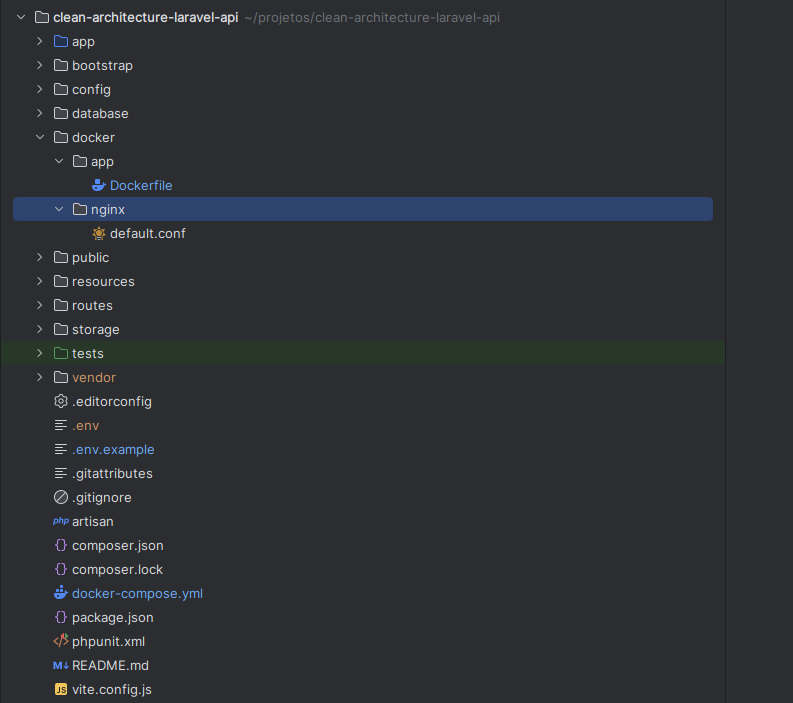
\includegraphics[width=0.9\textwidth]{figuras/tutorial/1estrutura.png}
            \caption{Estrutura de pastas do projeto}
            \label{fig:figura_tutorial_1}
            \newcommand{\minhafonteum}{Fonte: Autor}
            \minhafonteum
        \end{figure}

        \par O Dockerfile é o primeiro componente criado para o ambiente Docker, atuando como um ``manual de instruções'' para a construção da imagem do \textit{container} da aplicação. Ele utiliza a imagem base \texttt{php:8.2-fpm-alpine}, garantindo um ambiente leve e focado no processamento de scripts PHP. 

        \par Através de comandos RUN, o arquivo instala dependências essenciais, como o Git e bibliotecas de desenvolvimento, além de extensões PHP específicas, como a \texttt{pdo\_mysql}, que é necessária para a comunicação com o banco de dados. Por fim, o Dockerfile instala o Composer para gerenciar as dependências do Laravel e define o diretório de trabalho, garantindo que o contêiner esteja pronto para executar a aplicação. O Código \ref{lst:dockerfile} apresenta o código escrito no Dockerfile.

        \lstinputlisting[
            language=bash,
            inputencoding=utf8,
            caption={Código do Dockerfile.},
            label=lst:dockerfile,
            frame=single, % Adiciona uma moldura ao redor do código
            numbers=left, % Adiciona números de linha à esquerda
            breaklines=true, % Quebra linhas longas automaticamente
            basicstyle=\ttfamily\scriptsize % Define a fonte como monoespaçada e pequena
        ]{codigos/ca/docker/app/Dockerfile}

        \par O arquivo \texttt{default.conf}, localizado na pasta \texttt{docker/nginx}, é o responsável por configurar o servidor web Nginx. Sua principal função é atuar como um proxy reverso, recebendo todas as requisições HTTP e encaminhando-as para o \textit{container} da aplicação PHP.

        \par Dentro deste arquivo, a diretiva \texttt{root} é configurada para apontar para a pasta public do Laravel, que é o ponto de entrada da aplicação. A regra de \texttt{location /} garante que todas as requisições para URLs que não correspondem a arquivos existentes sejam redirecionadas para o \texttt{index.php} do Laravel, o que é fundamental para o sistema de roteamento do \textit{framework}.

        \par A seção \texttt{location \textasciitilde \textbackslash.php\$} é a mais crítica para o funcionamento da aplicação. Ela intercepta todas as requisições que terminam em .php e as encaminha para o serviço app (o \textit{container} PHP-FPM) na porta 9000. Essa configuração permite que o Nginx entregue arquivos estáticos diretamente e passe apenas as requisições dinâmicas para o PHP processar, otimizando o desempenho.

        \par No Código \ref{defaultconf} é apresentada a estrutura do arquivo \texttt{default.conf}.

        \lstinputlisting[
            language=bash,
            inputencoding=utf8,
            caption={Código do default.conf.},
            label=defaultconf,
            frame=single, % Adiciona uma moldura ao redor do código
            numbers=left, % Adiciona números de linha à esquerda
            breaklines=true, % Quebra linhas longas automaticamente
            basicstyle=\ttfamily\scriptsize % Define a fonte como monoespaçada e pequena
        ]{codigos/ca/docker/nginx/default.conf}

        \par O arquivo \texttt{docker-compose.yml} é o componente central para a orquestração do ambiente, atuando como um plano que define e gerencia os serviços da aplicação. Ele garante que cada serviço, como a aplicação Laravel, o servidor Nginx e o banco de dados MySQL, sejam criados e interligados corretamente, eliminando a complexidade de iniciar cada contêiner de maneira individual.

        \par Este arquivo é dividido em três seções principais:

        \begin{enumerate}
            \item \textbf{services}: Esta seção define os \textit{containers} que compõem a aplicação.
            \begin{itemize}
                \item \textbf{\texttt{app}}: Este serviço constrói o \textit{container} da aplicação, utilizando o \texttt{Dockerfile}. A diretiva \texttt{volumes} serve para que o código do projeto na máquina host seja sincronizado com o código dentro do \textit{container}.
                
                \item \textbf{\texttt{nginx}}: O \textit{container} do Nginx atua como um servidor web e \textit{proxy reverso}. Ele mapeia a porta \texttt{8000} da máquina host para a porta \texttt{80} do \textit{container}, permitindo que o acesso à aplicação pelo navegador.
                
                \item \textbf{\texttt{db}}: Este serviço cria o contêiner do MySQL. A diretiva \texttt{environment} configura o banco de dados com variáveis definidas no arquivo \texttt{.env}, enquanto a diretiva \texttt{volumes} garante a persistência dos dados. O mapeamento da porta \texttt{3307:3306} permite que o \textit{container} do banco de dados seja acessado na porta \texttt{3307} da máquina host, evitando conflitos com outras instalações do MySQL.
            \end{itemize}
        
            \item \textbf{networks}: Define uma rede virtual (\texttt{laravel-network}) que faz com que todos os serviços se comuniquem entre si de forma segura, usando seus nomes de serviço (\texttt{app}, \texttt{nginx}, \texttt{db}) como endereços.
        
            \item \textbf{volumes}: Gerencia a persistência dos dados do banco de dados, para que os dados não sejam perdidos quando o contêiner for parado ou recriado.
        \end{enumerate}
    
        \par No Código \ref{lst:figura.tutorial.4} é apresentado o conteúdo do arquivo \texttt{docker-compose.yml}.

        \lstinputlisting[
            language=bash,
            inputencoding=utf8,
            caption={Código do docker-compose.yml},
            label=lst:figura.tutorial.4,
            frame=single, % Adiciona uma moldura ao redor do código
            numbers=left, % Adiciona números de linha à esquerda
            breaklines=true, % Quebra linhas longas automaticamente
            basicstyle=\ttfamily\scriptsize % Define a fonte como monoespaçada e pequena
        ]{codigos/ca/docker-compose.yml}
        
    
        \par Após a configuração do ambiente Docker, o próximo passo foi preparar o ambiente de desenvolvimento da aplicação. Para isso, o arquivo \texttt{.env.example}, que contém um modelo das variáveis de ambiente padrão do projeto, precisou ser copiado e renomeado para \texttt{.env}. Esse arquivo é fundamental, pois armazena credenciais e configurações sensíveis, como chaves de acesso e informações de conexão com o banco de dados.

        \begin{sloppypar}
            \par É no arquivo .env que as variáveis como \texttt{DB\_CONNECTION}, \texttt{DB\_HOST}, \texttt{DB\_PORT},  \texttt{DB\_DATABASE}, \texttt{DB\_USERNAME}, \texttt{DB\_PASSWORD} e \texttt{DB\_ROOT\_PASSWORD} são ajustadas para corresponderem às configurações do serviço de banco de dados no arquivo docker-compose.yml. Isso permite que o \textit{container} da aplicação Laravel se conecte corretamente ao \textit{container} do banco de dados, estabelecendo a comunicação necessária para o funcionamento do projeto.
        \end{sloppypar}

        \begin{sloppypar}
            \par No Código \ref{lst:.env.example} é apresentado como ficou o parcialmente o arquivo \texttt{.env.example}, com as mudanças que são necessárias necessárias para o funcionamento da API REST, tal arquivo vai para o sistema controle de versão:
        \end{sloppypar}

        \lstinputlisting[
            language=bash,
            inputencoding=utf8,
            caption={Código do .env.example},
            label=lst:.env.example,
            frame=single, 
            numbers=left, 
            breaklines=true,
            basicstyle=\ttfamily\scriptsize
        ]{codigos/ca/.env.example}

        \par Após essa alteração foi rodado o seguinte comando no terminal para a criação do arquivo \texttt{.env}, o qual não estará disponível no sistema de controle de versão:

        \begin{verbatim}
        cp .env.example .env
        \end{verbatim}

        \par Após o ambiente estar com as variáveis configuradas pôde-se rodar o seguinte comando:

        \begin{verbatim}
        docker-compose up -d --build
        \end{verbatim}

        \par O comando \texttt{docker-compose up -d --build} é a ferramenta central para a orquestração do ambiente de desenvolvimento, unificando três ações essenciais em uma única instrução. A diretiva up inicia todos os serviços definidos no arquivo \texttt{docker-compose.yml}, como a aplicação Laravel, o servidor web Nginx e o banco de dados MySQL. 
        
        \par A flag \texttt{-d} (modo detached) executa esses \textit{containers} em segundo plano, liberando o terminal para outras atividades. Por fim, a flag \texttt{--build} garante que as imagens dos \textit{containers} sejam reconstruídas a partir dos arquivos Dockerfile antes de serem iniciadas, assegurando que o ambiente esteja sempre atualizado com as últimas modificações no código-fonte ou nas dependências.

        \par Em seguida foi rodado o seguinte comando:

        \begin{verbatim}
        docker-compose exec app php artisan key:generate
        \end{verbatim}

        \par O comando \texttt{docker-compose exec app php artisan key:generate} é fundamental para a configuração inicial do Laravel. A instrução docker-compose exec permite executar comandos diretamente dentro de um contêiner em execução, neste caso, o serviço app que representa a aplicação.
        
        \par O \texttt{php artisan key:generate} é um comando do Laravel que gera uma chave de segurança única. Essa chave é usada para criptografar sessões, cookies e outras informações sensíveis da aplicação, sendo um passo essencial para garantir a segurança e o correto funcionamento do projeto.

        \par A última etapa da configuração do ambiente foi a execução do seguinte comando, para rodar as migrações do Laravel dentro do \textit{container} da aplicação:
        
        \begin{verbatim}
        docker-compose exec app php artisan migrate
        \end{verbatim}
        
        \sloppy
        \par Após essas etapas, o ambiente Docker foi verificado com o comando \texttt{docker-compose ps}, o qual demonstrou sucesso na execução dos contêineres. Em seguida, foi realizada a validação da execução da aplicação, acessando a URL \textbf{http://localhost:8000/}.
        
    \subsection{Codificação da API REST}
    
        \par Esta etapa tem como objetivo descrever o processo de codificação da API REST seguindo o tutorial do PET, levando em consideração que o projeto com o \textit{framework} Laravel e o ambiente de desenvolvimento com Docker já estão organizados e rodando.
        
        \par Inicialmente, foi realizada a criação do Model e da Migration. O Model é responsável por representar a entidade \textit{Contact} do banco de dados dentro da aplicação, enquanto a Migration define a configuração da tabela que irá armazenar esse recurso. Para isso, foi executado o seguinte comando do Artisan:

        \begin{verbatim}
        docker-compose exec app php artisan make:model Contact -m
        \end{verbatim}
        
        \par Ao rodar esse comando, foram criados dois arquivos, \textit{app/Models/Contact.php}, correspondente ao Model, e um arquivo com final \texttt{create\_contacts\_table}, localizado em \texttt{database/migrations}, que corresponde à Migration. 

        \par Conforme mostra o Código~\ref{lst:mvc-model-0}, arquivo referente ao Model apresenta a seguinte implementação:

        \lstinputlisting[
            language=PHP,
            inputencoding=utf8,
            caption={Código do Model},
            label=lst:mvc-model-0,
            frame=single, 
            numbers=left, 
            breaklines=true,
            basicstyle=\ttfamily\scriptsize
        ]{codigos/api-pet/Contact.php}

        \par Conforme apresenta o Código~\ref{lst:mvc-migration-0}, o arquivo de Migration ficou estruturado da seguinte forma:

        \lstinputlisting[
            language=PHP,
            inputencoding=utf8,
            caption={Código da Migration},
            label=lst:mvc-migration-0,
            frame=single,
            numbers=left,
            breaklines=true,
            basicstyle=\ttfamily\scriptsize
        ]{codigos/api-pet/Migration.php}

        \par Em seguida, foi necessário alterar o arquivo \texttt{bootstrap/app.php} para registrar o arquivo de rotas da API. O Código~\ref{lst:mvc-app-0} apresenta a nova configuração aplicada:
        
        \lstinputlisting[
            language=PHP,
            inputencoding=utf8,
            caption={Configuração do arquivo \texttt{bootstrap/app.php}},
            label=lst:mvc-app-0,
            frame=single,
            numbers=left,
            breaklines=true,
            basicstyle=\ttfamily\scriptsize
        ]{codigos/api-pet/app.php}

        \par Após o registro no arquivo \texttt{bootstrap/app.php}, foi criado o arquivo de rotas \texttt{routes/api.php}, no qual foram definidas as rotas da API. O Código~\ref{lst:mvc-routes-api-0} apresenta a implementação final desse arquivo:
        
        \lstinputlisting[
            language=PHP,
            inputencoding=utf8,
            caption={Arquivo de rotas \texttt{routes/api.php}},
            label=lst:mvc-routes-api-0,
            frame=single,
            numbers=left,
            breaklines=true,
            basicstyle=\ttfamily\scriptsize
        ]{codigos/api-pet/api.php}

        \sloppy

        \par O último arquivo a ser criado foi o \texttt{ContactController.php}, localizado em \texttt{app/Http/Controllers}. O Código~\ref{lst:mvc-controller-0} apresenta o conteúdo final desse arquivo:

        \vspace{1cm}
        
        \lstinputlisting[
            language=PHP,
            inputencoding=utf8,
            caption={Arquivo \texttt{ContactController.php}},
            label=lst:mvc-controller-0,
            frame=single,
            numbers=left,
            breaklines=true,
            basicstyle=\ttfamily\scriptsize
        ]{codigos/api-pet/ContactController.php}

        \par O arquivo \texttt{ContactController.php} implementa o Controller responsável pelo gerenciamento das operações relacionadas à entidade \textit{Contato}. Ele define métodos para criar (\texttt{store}), listar (\texttt{index}), exibir um registro específico (\texttt{show}), atualizar (\texttt{update}) e deletar (\texttt{destroy}) contatos no banco de dados, utilizando o Model \texttt{Contact}. 
        
        \par Cada método realiza a operação correspondente dentro de um bloco \texttt{try/catch}, retornando um array indicando sucesso ou, em caso de falha, o erro ocorrido. Esse Controller permite, portanto, a manipulação completa dos dados de contatos através das rotas da API.

    \section{Implementação da Arquitetura Limpa}

    \par Esta seção descreve a aplicação dos princípios propostos por \cite{livro:martin:cleanarch} na API REST de contatos desenvolvida pelo grupo PET. Inicialmente, apresenta-se uma análise comparativa entre o cenário típico da Arquitetura Limpa, conforme definido por \cite{livro:martin:cleanarch}, e o modelo arquitetural Model-View-Controller (MVC) utilizado nativamente pelo \textit{framework} Laravel. Em seguida, procede-se à reorganização da aplicação segundo as camadas da Arquitetura Limpa, de modo a evidenciar a adaptação prática do modelo teórico ao contexto do presente estudo.

    \subsection{Camada de Entidades}

        \par O primeiro passo prático na refatoração da API REST de contatos para a Arquitetura Limpa consiste em estabelecer seu núcleo. Conforme a abordagem proposta por \cite{livro:martin:cleanarch}, a camada mais interna e fundamental de um sistema é a das Entidades.

        \par Para a API de Contatos, a entidade principal é a Contact. Seguindo os princípios da Arquitetura Limpa, esta entidade não deve ter qualquer acoplamento com o Eloquent ORM do Laravel. Em vez disso, ela será uma classe PHP pura. A principal responsabilidade desta classe é representar um contato e suas regras intrínsecas, garantindo a integridade de seus dados.

        \par Nesse cenário, o arquivo \texttt{app/Entities/Contact.php} define a classe que representa a entidade. Primeiramente, foram definidas as propriedades e o construtor da classe com as chamadas para os métodos \texttt{setters}, conforme o código abaixo demonstra:

        \lstinputlisting[language=PHP, inputencoding=utf8]{codigos/clean_arch/entidade_construtor.php}

        \par Em seguida, na mesma classe foram criados os método \texttt{getters} e \texttt{setters}, conforme o código abaixo:
        
        \lstinputlisting[language=PHP, inputencoding=utf8]{codigos/clean_arch/entidade_getter_setter.php}

        \par Além da implementação dessas propriedades e métodos, nota-se na entidade o modificador \texttt{final}, fazendo com que a classe não possa ser estendida, garantindo que o núcleo da aplicação permaneça independente, já que é uma entidade base que vai ser usada pelos casos de uso.
        
        \par Cada método \texttt{setter} pode ter uma validação específica para garantir a consistência e a integridade de um contato. Esta classe não possui conhecimento sobre como será persistida no banco de dados ou como será exibida em uma resposta HTTP, cumprindo o principal objetivo da Arquitetura Limpa de isolar o núcleo do sistema.

    \subsection{Camada de Casos de Uso}
\label{sec:casos_de_uso}

    \par Conforme a abordagem proposta por \cite{livro:martin:cleanarch}, a camada de Casos de Uso é responsável por conter as regras de negócio específicas da aplicação, orquestrando as Entidades para executar as ações que o sistema oferece. Para a API de contatos, as operações de CRUD (\textit{Create, Read, Update, Delete}) foram mapeadas para Casos de Uso individuais, garantindo a coesão e a separação de responsabilidades.


    
        \par A estrutura de diretórios foi organizada de modo a isolar cada caso de uso em sua própria pasta, como \texttt{app/UseCases/CreateContact/} e \texttt{app/UseCases/UpdateContact/}. Essa abordagem reflete o conceito de `Arquitetura Gritante'' (MARTIN, 2019), onde a estrutura do projeto por si só deve comunicar suas funcionalidades. Para refinar ainda mais a organização, foram criadas subpastas para agrupar os diferentes tipos de componentes dentro de cada caso de uso:
        
            \begin{itemize}
                \item \texttt{Boundaries/}: Agrupa as interfaces que definem os contratos de entrada (\textit{InputBoundary}) e saída (\textit{OutputBoundary}) do caso de uso.
                
                \item \texttt{DTOs/}: Contém os \textit{Data Transfer Objects}, estruturas de dados responsáveis por transportar informações através das \textit{boundaries}.
                
                \item \texttt{Interactor}: A classe principal que contém a implementação da lógica de negócio.
            \end{itemize}

        \par Após a criação da estrutura dos casos de uso, foi criada uma Interface para representar a \texttt{DataAccessInterface}, essa interface representa a implementação do \texttt{DataAccess} da camada de Frameworks e Drivers. Para realizar esse isolamento do acesso ao banco de dados, foi utilizado o padrão RepositoryPattern, onde tem-se uma classe que implementa as operações de acesso ao banco de dados, e uma interface que fica na camada de Casos de Uso.

        \par Para aderir a esse padrão, foi criada a Interface \texttt{ContactRepositoryInterface} (Código \ref{lst:contact.repo.interface})  dentro do diretório \texttt{app/UsesCases/Contracts}, essa interface apenas define os métodos que vão ser usados pelos casos de uso, essa Interface faz com que essa camada não conheça qual banco de dados ou ORM a aplicação usa, assim aderindo à inversão de dependência.

        \lstinputlisting[language=PHP, inputencoding=utf8, caption={Interface do repositório de Contatos.}, label=lst:contact.repo.interface]{codigos/clean_arch/casos_de_uso/ContactRepositoryInterface.php}
    
        \par Para exemplificar a implementação, o caso de uso \texttt{CreateContact} é detalhado a seguir, por ser o mais completo na aplicação do padrão, demonstrando a função de cada componente.
        
        \par Os primeiros elementos a serem criados são os DTOs, eles são classes simples, responsáveis por transportar dados de forma estruturada. São definidos dois DTOs: um para a requisição (\texttt{RequestModel}), que carrega os dados de entrada, e um para a resposta (\texttt{ResponseModel}), que carrega os dados de saída do caso de uso. Essas classes dentro da representação de \cite{livro:martin:cleanarch} de um cenário típico da arquitetura limpa, são representados pelos componentes \texttt{InputData} e  \texttt{OutputData}.
        
        \lstinputlisting[language=PHP, inputencoding=utf8, caption={DTO de Requisição para o Caso de Uso de Criação.}, label=lst:create.request.model]{codigos/clean_arch/casos_de_uso/CreateContactRequestModel.php}
        
        \lstinputlisting[language=PHP, inputencoding=utf8, caption={DTO de Resposta para o Caso de Uso de Criação.}, label=lst:create.response.model]{codigos/clean_arch/casos_de_uso/CreateContactResponseModel.php}
        
        \par As \textit{boundaries} representam os contratos que garantem a inversão de dependência. A \texttt{InputBoundary} (Código \ref{lst:create.input.boundary}) define a porta de entrada do caso de uso, servindo como uma abstração que será implementada pelo \texttt{Interactor} e consumida pelo \texttt{Controller}.
        
        \lstinputlisting[language=PHP, inputencoding=utf8, caption={Input Boundary para o Caso de Uso de Criação.}, label=lst:create.input.boundary]{codigos/clean_arch/casos_de_uso/CreateContactInputBoundary.php}
        
        \par  Já a \texttt{OutputBoundary} (Código \ref{lst:create.output.boundary}) define o contrato para a camada de apresentação, sendo implementada pelo \texttt{Presenter}.
        
        \lstinputlisting[language=PHP, inputencoding=utf8, caption={Output Boundary para o Caso de Uso de Criação.}, label=lst:create.output.boundary]{codigos/clean_arch/casos_de_uso/CreateContactOutputBoundary.php}
        
        
        \par O Interactor (Código \ref{lst:create.interactor}) é a classe que contém a lógica de negócio pura. Ele implementa a \texttt{InputBoundary} e orquestra a interação com as Entidades, utilizando outras abstrações — como a \texttt{ContactRepositoryInterface} e a \texttt{CreateContactOutputBoundary} — para se comunicar com as camadas externas sem conhecê-las diretamente.
        
        
        \lstinputlisting[language=PHP, inputencoding=utf8, caption={Estrutura do Interactor de Criação de Contato.}, label=lst:create.interactor]{codigos/clean_arch/casos_de_uso/CreateContactInteractor.php}

        \par No (Código \ref{lst:create.interactor.create}) tem-se a implementação do método create do \texttt{Interactor}, esse método realiza a regra de negócio do caso de uso, como as validações e etapas necessárias para a criação de um Contato. Esse método recebe os dados pela estrutura de dados de entrada e ao final retorna o método \texttt{present()} da interface \texttt{CreateContactOutputBoundary}, que é a representação do \texttt{Presenter}. Desse modo o caso de uso não conhece as implementações das outras camadas, mantendo os princípios da Arquitetura Limpa.

        \lstinputlisting[language=PHP, inputencoding=utf8, caption={Estrutura do método create do Interactor de Criação de Contato.}, label=lst:create.interactor.create]{codigos/clean_arch/casos_de_uso/CreateContactInteractor@create.php}
        
        \par As implementações completas para as demais operações de CRUD seguem os mesmos princípios aqui demonstrados, variando apenas na complexidade de seus DTOs e na lógica de seus Interactors. Para fins de brevidade, seus códigos não serão detalhados neste documento, mas podem ser consultados na íntegra no repositório do projeto no GitHub.





    \chapter{MVC versus Arquitetura Limpa}

    \par Este capítulo apresenta uma comparação entre a API REST original desenvolvida em MVC e sua versão refatorada com Arquitetura Limpa. A análise destaca as principais mudanças na estrutura do projeto e no fluxo das requisições, estabelecendo uma base para a compreensão dos resultados apresentados nas seções seguintes. Dessa forma, busca-se proporcionar uma visão geral da refatoração, evidenciando os impactos e aspectos que devem ser considerados na adoção da Arquitetura Limpa, os quais serão discutidos posteriormente neste trabalho.

    \par Para essa avaliação, foram definidos alguns critérios, baseados nas preocupações que motivaram a Arquitetura Limpa. Os fatores definidos para evidenciar as diferenças e semelhanças entre as abordagens são: Estrutura e Organização (que avalia o conceito de "Arquitetura Gritante" e a clareza de diretórios), Acoplamento e Coesão (medido pela aderência à Regra da Dependência e o isolamento do núcleo de negócio), Fluxo da Requisição (analisando o caminho e o número de responsabilidades por componente), e a Testabilidade/Flexibilidade (a capacidade de trocar detalhes de infraestrutura sem afetar a lógica central).
    
    \section{Comparação Estrutural}
        \par Para apresentar a materialização do modelo conceitual proposto por \cite{livro:martin:cleanarch}, a Tabela \ref{tab:mapeamento_clean_arch} apresenta o mapeamento direto entre cada componente teórico apresentado pelo autor e a sua respectiva representação no projeto, utilizando o caso de uso de criação de um novo contato como exemplo.
        
        \begin{table}[H]
            \caption{Mapeamento dos Componentes}
            \label{tab:mapeamento_clean_arch}
            \begin{tabularx}{\linewidth}{|l|X|} % Adicionados os "|" para as linhas verticais
                \toprule
                % A linha do cabeçalho foi envolvida por {\small ...} para diminuir a fonte
                {\small \textbf{Componente no Cenário Típico (Martin, 2019)}} & {\small \textbf{Classe/Artefato Implementado no Projeto}} \\
                \midrule
                Controller                  & \texttt{CreateContactController.php} \\
                Input Boundary (Interface)  & \texttt{CreateContactInputBoundary.php} \\
                Use Case Interactor         & \texttt{CreateContactInteractor.php} \\
                Input Data                  & \texttt{CreateContactRequestModel.php} \\
                Entities                    & \texttt{Contact.php} (Entidade Pura) \\
                Data Access Interface       & \texttt{ContactRepositoryInterface.php} \\
                Data Access (Implementação) & \texttt{ContactRepository.php} \\
                Database                    & MySQL (Serviço Docker) \\
                Output Boundary (Interface) & \texttt{CreateContactOutputBoundary.php} \\
                Presenter                   & \texttt{CreateContactApiPresenter.php} \\
                Output Data                 & \texttt{CreateContactResponseModel.php} \\
                View Model                  & \texttt{ContactViewModel.php} \\
                View                        & Resposta JSON \\
                \bottomrule
            \end{tabularx}
        \end{table}
       
        \par Essa tradução da teoria para a prática se inicia com o Controller, representado pela classe \texttt{CreateContactController.php}, que transforma a requisição em um Input Data, implementado como o DTO \texttt{CreateContactRequestModel.php}. Este objeto é então passado para o Use Case Interactor (\texttt{CreateContactInteractor.php}) através da Input Boundary, o contrato definido pela interface \texttt{CreateContactInputBoundary.php}. No núcleo da aplicação, o Interactor orquestra as Entities, materializadas pela classe pura \texttt{Contact.php}. 
        
        \par A persistência dos dados é abstraída pela Data Access Interface (\texttt{ContactRepositoryInterface.php}), cuja implementação concreta é o \texttt{ContactRepository.php}, que por sua vez interage com o Database (MySQL). Ao final do fluxo, o Interactor produz o Output Data (\texttt{CreateContactResponseModel.php}) e o entrega ao Presenter (\texttt{CreateContactApiPresenter.php}) através da Output Boundary (\texttt{CreateContactOutputBoundary.php}). Por fim, o Presenter formata esses dados em um View Model (\texttt{ContactViewModel.php}), que serve de base para a View, representada pela Resposta JSON final.

        \par Apresentados os componentes resultantes da aplicação da Arquitetura Limpa, pode-se realizar uma comparação entre a arquitetura MVC e a Arquitetura Limpa no contexto desse TCC, apresentando as diferenças entre a abordagem inicial, centrada no framework, e a abordagem final, centrada no domínio de negócio. 
        
        \par A primeira mudança perceptível está na organização dos diretórios. A estrutura MVC original agrupa os arquivos por seu tipo técnico (Models, Controllers), enquanto a nova estrutura os organiza por camadas e funcionalidades, refletindo o conceito de "Arquitetura Gritante".
        
        \par Nesse sentido, nota-se que a API base, seguindo o padrão Laravel, possuía uma estrutura enxuta, com a lógica de negócio, acesso a dados e controle de requisições concentradas principalmente nos diretórios \texttt{app/Http/Controllers} e \texttt{app/Models}, conforme consta na Figura~\ref{fig:estrutura-original} onde é apresentada a estrutura do diretório \texttt{app} da API REST base. 

        \begin{figure}[H]
            \caption{Estrutura do diretório app antes da refatoração.}
            \label{fig:estrutura-original}
            \dirtree{%
            .1 app/.
            .2 Http/.
            .3 Controllers/.
            .4 ContactController.php.
            .4 Controller.php.
            .2 Models/.
            .3 Contact.php.
            .3 User.php.
            .2 Providers.
            .3 AppServiceProvider.php.
            }
        \end{figure}

        \par Já após a refatoração, a estrutura de diretórios passou a refletir as camadas da Arquitetura Limpa. As regras de negócio agora residem em \texttt{app/Entities} e \texttt{app/UseCases}, completamente isoladas do framework. Os componentes que interagem com o mundo externo, como Controllers e Repositories, foram movidos para \texttt{app/InterfaceAdapters}, e os detalhes de implementação específicos do Laravel, como os Models do Eloquent, para \texttt{app/FrameworksAndDrivers}. A Figura \ref{fig:estrutura-depois} demonstra a organização final do diretório \texttt{app}.

        \begin{figure}[H]
            \caption{Estrutura do diretório app após a refatoração.}
            \label{fig:estrutura-depois}
            \dirtree{%
            .1 /app.
            .2 Entities.
            .3 Contact.php.
            .2 FrameworksAndDrivers.
            .3 Models.
            .4 ContactModel.php.
            .3 Providers.
            .4 AppServiceProvider.php.
            .4 CleanArchServiceProvider.php.
            .2 InterfaceAdapters.
            .3 Http.
            .4 Controllers.
            .5 Controller.php.
            .5 Contact.
            .6 CreateContactController.php.
            .6 ....
            .3 Presenters.
            .4 Api.
            .5 CreateContactApiPresenter.php.
            .5 ....
            .3 Repositories.
            .4 ContactRepository.php.
            .3 ViewModels.
            .4 ContactViewModel.php.
            .2 UseCases.
            .3 Contracts.
            .4 ContactRepositoryInterface.php.
            .3 CreateContact.
            .4 CreateContactInteractor.php.
            .4 Boundaries.
            .5 CreateContactInputBoundary.php.
            .5 CreateContactOutputBoundary.php.
            .4 DTOs.
            .5 CreateContactRequestModel.php.
            .5 CreateContactResponseModel.php.
            .3 Exceptions.
            .4 BusinessRuleException.php.
            .4 ResourceNotFoundException.php.
            .3 ....
        }
        \end{figure}

        \par Essa nova organização deixa explícito o propósito da aplicação (gerenciar contatos, com casos de uso como CreateContact, etc.) antes mesmo de revelar qual tecnologia é usada para isso.

    \section{Comparação do fluxo da Requisição}

    \par O fluxo da Arquitetura MVC Original, ilustrado na Figura~\ref{fig:mvc1}, é direto e revela um alto nível de acoplamento ao \textit{framework}, violando o Princípio da Responsabilidade Única. A requisição HTTP (\texttt{POST /contacts}) é recebida pela Rota, que a encaminha ao \texttt{ContactController}. O \textit{Controller} é então ativado e assume múltiplas responsabilidades simultaneamente: ele instancia diretamente o \texttt{ContactModel} (Eloquent), criando um forte acoplamento ao ORM, e define seus atributos com os dados brutos da requisição HTTP. 
    
    \par Em seguida, o \textit{Controller} chama o método \texttt{save()} do \textit{Model}, orquestrando a persistência de dados no Banco de Dados. Esse comportamento fez com que o \textit{Controller} atue como manipulador de HTTP, orquestrador de lógica de negócio e componente de acesso a dados. O fluxo é finalizado com o \textit{Controller} retornando a resposta JSON ao Cliente, acumulando também a responsabilidade de formatação da saída (\textit{Presenter}).

    \par Com a refatoração, o fluxo (Figura~\ref{fig:ca1}) inverte as dependências, garantindo que o núcleo da aplicação seja totalmente isolado. O processo começa com o \texttt{Controller} (Adaptador de Interface) recebendo a requisição HTTP (1). Seu papel é estritamente limitado à tradução da entrada: ele cria o \texttt{RequestModel} (DTO) (2) e invoca o Caso de Uso através da interface \texttt{InputBoundary} (3), passando o DTO agnóstico e uma instância do \texttt{Presenter}.

    \par O \texttt{Interactor} (Caso de Uso) é ativado na camada de lógica de negócio. Sua responsabilidade é puramente a execução da regra: ele cria e valida a \texttt{Entidade Contact} (4) e, para persistir, chama a \texttt{ContactRepositoryInterface} (5). A Regra da Dependência é estritamente obedecida, pois o \textit{Interactor} não conhece o \textit{framework} ou o ORM. A implementação concreta do repositório interage com o Banco de Dados (6, 7, 8) e retorna a \texttt{Entidade Salva} para o \textit{Interactor}.

    \par O \texttt{Interactor} cria o \texttt{ResponseModel} (DTO de saída) (9) e o envia ao \texttt{Presenter} através da \texttt{OutputBoundary} (10), finalizando a lógica de negócio. O \texttt{Presenter} (Adaptador de Saída) formata os dados brutos no \texttt{ViewModel} (11). O \texttt{Controller} (Adaptador de Entrada) recupera o \texttt{ViewModel} (13, 14) e envia a resposta JSON (15). Essa segregação de tarefas, ao isolar a lógica de negócio na camada de \textit{Use Cases}, torna o núcleo da aplicação totalmente testável em unidade (sem dependência do \textit{framework}, \textit{HTTP} ou Banco de Dados) e flexível a alterações de tecnologia externa.

    \begin{figure}[H]
        \centering
    
        \begin{minipage}{0.49\linewidth}
            \centering
            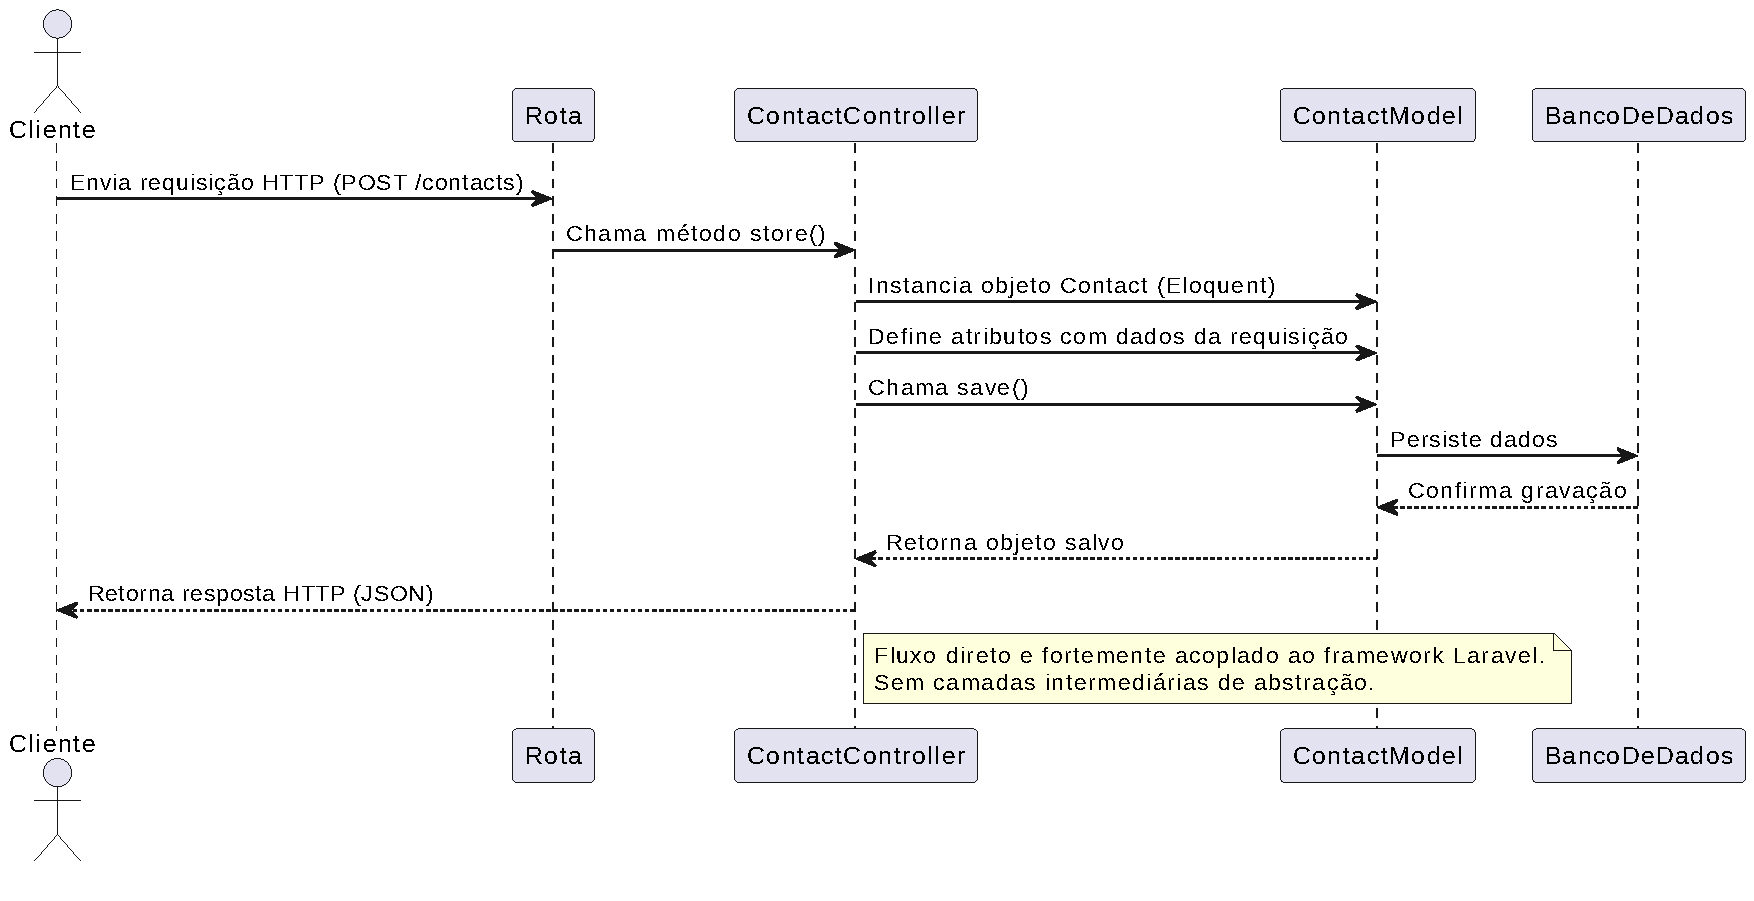
\includegraphics[angle=-90,width=1.0\linewidth]{figuras/resultados/mvc1.pdf}
            \caption{Fluxo da Requisição - Arquitetura MVC Original (Laravel).}
            \label{fig:mvc1}
            
        \end{minipage}
        \hfill
        \begin{minipage}{0.49\linewidth}
            \centering
            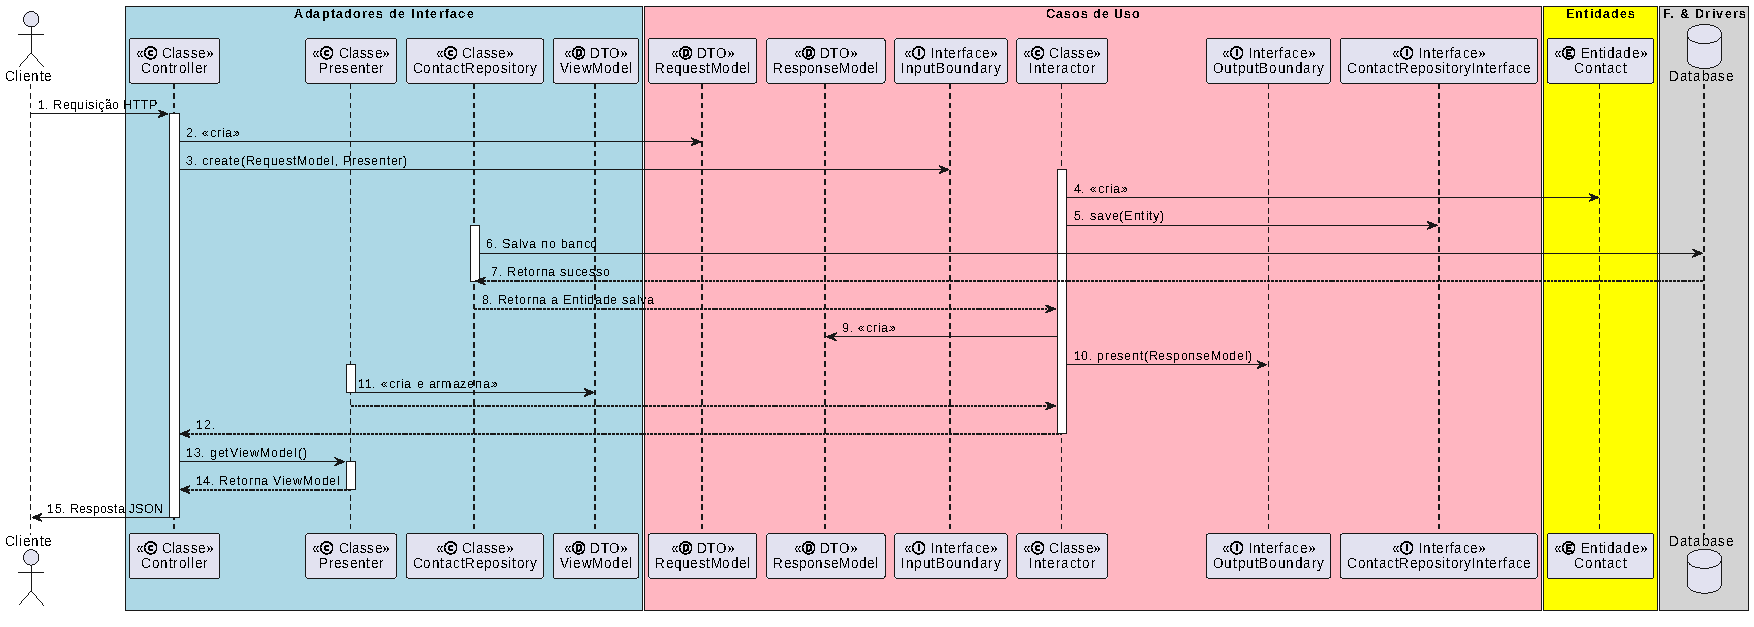
\includegraphics[angle=-90,width=1.0\linewidth]{figuras/resultados/ca1.pdf}
            \caption{Fluxo da Requisição - Arquitetura Limpa (Laravel).}
            \label{fig:ca1}
            
        \end{minipage}
    \end{figure}

    \vspace{1cm}


    \par Diante dessa comparação, pode-se notar que o padrão MVC não foi descartado, mas sim reposicionado. No modelo original da API REST no Laravel, o Controller e o Model atuavam de forma acoplada, concentrando tanto a adaptação da requisição HTTP, quanto a lógica de negócio e a persistência de dados.

    \par Diferentemente, com a Arquitetura Limpa, essa concentração de responsabilidades foi desmembrada e realocada, alinhando-se aos princípios SOLID e à Regra da Dependência. O Controller foi movido para a camada de Adaptadores de Interface, assumindo a única função de traduzir a requisição HTTP em um RequestModel (DTO) e invocar o Caso de Uso correspondente.

    \par Já o Model foi isolado na camada mais externa de Frameworks e Drivers, enquanto sua lógica essencial de domínio foi migrada para a classe pura da Entidade (Contact.php) e para o Interactor, que representa o novo núcleo de negócio (Caso de Uso).

    \par O resultado é que o padrão MVC passou a operar estritamente como a camada de interação externa, adaptando as entradas e saídas (com o auxílio do Presenter e ViewModel para a View JSON), enquanto o núcleo de negócio permanece completamente isolado e agnóstico ao framework.
    \chapter{Resultados e Discussões}
\thispagestyle{headings}

    \par As implicações dessas alterações são profundas, tanto em termos de implementações novas quanto de manutenibilidade. No que tange à implementação, a nova abordagem exige uma estrutura de código mais elaborada. A criação de uma única funcionalidade, que antes se resumia a um método em um Controller, agora envolve a definição de Entidades, Casos de Uso com seus respectivos DTOs e Boundaries, e as implementações dos adaptadores, como o Repository e o Presenter.
    
    \par É notável que embora isso represente um aumento na quantidade de arquivos e na complexidade inicial, a implementação passa a ser guiada por contratos (interfaces), reforçando o Princípio da Inversão de Dependência e resultando em um código mais explícito e coeso. É na manutenibilidade, no entanto, que os maiores benefícios serão percebidos, sendo este um dos objetivos centrais da Arquitetura Limpa. Ao isolar o núcleo da aplicação (Casos de Uso e Entidades) dos detalhes de infraestrutura como o \textit{framework} e o banco de dados, a arquitetura facilita a manutenção futura. 
    
    \par Na prática, a substituição do Eloquent ORM por outra ferramenta de persistência, por exemplo, exigiria apenas a criação de uma nova classe que implemente a ContactRepositoryInterface, sem qualquer alteração na lógica de negócio contida no Interactor. Essa separação estrita de interesses não só protege as regras de negócio de mudanças em tecnologias externas, mas também pode tornar o sistema mais flexível e testável.
    
    \par Contudo, é fundamental aprofundar a discussão sobre os \textit{trade-offs} (compensações) envolvidos nessa adoção, que vão além da implementação técnica e afetam diretamente a dinâmica da equipe de desenvolvimento, o ciclo de vida do projeto e a alocação de recursos.
    
    \par Um desses desafios é a curva de aprendizado e a integração da equipe. Na adoção da Arquitetura Limpa em um ecossistema como o Laravel, a dificuldade imposta ao time é evidente. A estrutura nativa do \textit{framework} é amplamente conhecida e documentada, e sua filosofia de ``convenção sobre configuração'' permite que desenvolvedores, mesmo com menos experiência, se tornem produtivos rapidamente e saibam onde encontrar cada componente do sistema. 
    
    \par Contudo, essa facilidade inicial não garante que o código esteja bem organizado: pois pode ser possível encontrar regras de negócio profundamente acopladas aos \textit{Controllers}, validações misturadas com lógica de apresentação, e dependências diretas do \textit{Eloquent} espalhadas por toda a aplicação. Principalmente em projetos onde não houve uma preocupação com arquitetura desde o inicio.
    
    \par Ao adotar a Arquitetura Limpa, o projeto se desvia significativamente dessa convenção em favor de uma organização mais rígida e explícita. Profissionais com pouco ou nenhum conhecimento prévio em \textit{design} de \textit{software} orientado a camadas, SOLID e padrões de projeto (como \textit{Repository}, DTOs e \textit{Data Mappers}) podem encontrar uma dificuldade inicial considerável.

    \par Isso implica que a integração de novos membros à equipe (processo de \textit{onboarding}) exigirá um período de treinamento e mentoria mais longo. A equipe precisa não apenas entender o domínio de negócio, mas também a filosofia arquitetural do projeto, que agora possui suas próprias convenções, independentes do \textit{framework}.
    
    \par Outro ponto de análise é o custo de desenvolvimento de novas funcionalidades. Conforme apontado, a complexidade inicial e o aumento no número de arquivos refletem-se diretamente no tempo de desenvolvimento. A implementação de uma nova tarefa ou melhoria, por menor que seja, exigirá um esforço inicial maior. 
    
    \par A criação de um novo \textit{endpoint} de CRUD, por exemplo, que no MVC padrão do Laravel poderia ser resumida a um ou dois métodos no \textit{Controller} e ajustes no \textit{Model}, agora demanda a criação de uma cadeia de artefatos: a definição (ou reutilização) da Entidade, a criação do Caso de Uso (\textit{Interactor}), a definição das \textit{Boundaries} (entrada e saída), a criação dos DTOs (\textit{Request} e \textit{Response}), a implementação do \textit{Controller} e do \textit{Presenter} (como Adaptadores), a atualização da interface do Repositório (se necessário) e, por fim, a implementação no Repositório concreto.
    
    \par Esse ``\textit{boilerplate}'' (código repetitivo) de infraestrutura arquitetural, embora garanta o desacoplamento, inevitavelmente torna o ciclo de desenvolvimento de novas \textit{features} mais lento. Este é um custo que deve ser conscientemente aceito pela equipe e pelo negócio em troca dos benefícios de longo prazo.
       
    \par Deve-se considerar, também, a aplicação em projetos legados e de alta complexidade. O presente estudo de caso partiu de uma API REST base relativamente simples. A transposição dessa metodologia para um sistema de \textit{software} em produção, especialmente um projeto legado ou de alta complexidade, é um desafio de outra magnitude.
    
    \par Em sistemas legados, o acoplamento profundo das regras de negócio com o \textit{framework} (especialmente com o Eloquent) é comum. A tentativa de refatorar um sistema nessas condições pode ser paralisante e introduzir um alto risco de geração de novos bugs. Nesses cenários, a implementação da Arquitetura Limpa provavelmente exigiria uma equipe dedicada e uma estratégia de migração gradual, onde novas funcionalidades são construídas seguindo a nova arquitetura e funcionalidades antigas são refatoradas incrementalmente. O custo e o tempo para essa transição seriam significativamente maiores, podendo justificar a alocação de uma equipe específica apenas para essa modernização arquitetural.
    
    \par Em contrapartida direta ao aumento do custo de implementação, a arquitetura oferece vantagens claras na manutenibilidade, testabilidade e na resolução de bugs. A principal vantagem reside na testabilidade aprimorada, um dos pilares da arquitetura.
    
    \par O isolamento rigoroso do \textit{Interactor} (camada de Casos de Uso) permite a criação de testes unitários robustos que validam a lógica de negócio pura, sem a necessidade de simular o \textit{framework}, requisições HTTP ou conexões com o banco de dados. As dependências externas (como o repositório) são injetadas via interfaces, permitindo o uso de dublês de teste de forma mais fácil.
    
    \par Essa cobertura de testes na camada mais crítica do sistema facilita a rápida identificação e localização precisa de falhas. Quando um \textit{bug} é reportado, pode ser mais fácil diagnosticá-lo: a falha está na tradução de dados feita pelo \textit{Controller}? Está na formatação do \textit{Presenter}? Ou está na regra de negócio dentro do \textit{Interactor}? Como o \textit{Interactor} é puramente testável, ele pode ser validado ou descartado como fonte do problema rapidamente, tornando o processo de \textit{debugging} mais eficiente e rápido.

    \par Em suma, para que uma equipe de desenvolvimento ou uma empresa decida adotar a Arquitetura Limpa, é fundamental avaliar o \textit{trade-off} entre o custo inicial de complexidade e o ganho de longevidade. Essa análise de viabilidade deve ser ancorada em três fatores críticos: a complexidade do projeto, o tamanho e a experiência da equipe, e a necessidade de mudança.

    \par O primeiro fator é a complexidade do projeto. A arquitetura é idealmente indicada para sistemas de alta complexidade, a qual se caracteriza por ter alta volatilidade nas regras de negócio e uma expectativa de longevidade a longo prazo (tipicamente, cinco anos ou mais). Para projetos de escopo simples, que demandam agilidade imediata, o custo de \textit{boilerplate} não se justifica. Nesses casos, o benefício da manutenibilidade é ofuscado pelo alto custo de desenvolvimento inicial, pois o tempo gasto na criação das múltiplas camadas de adaptação e interfaces consome recursos que seriam melhor utilizados na entrega rápida de \textit{features} através de um modelo mais simples, como o MVC nativo.
    
    \par O segundo fator é o tamanho e a experiência da equipe. Equipes grandes, ou aquelas que enfrentam alta rotatividade de membros, apresentam um cenário particularmente favorável à Arquitetura Limpa. Embora o processo de \textit{onboarding} demande um tempo inicial maior para compreensão dos conceitos arquiteturais, a clareza estrutural compensa essa complexidade ao oferecer um mapa mental consistente do sistema.
    
    \par Um exemplo disso pode ser a saída de um membro experiente, que não ``leva'' consigo a organização e as regras de funcionamento de uma parte do sistema desenvolvida por ele, tornando a substituição de membros mais segura, ainda que exija treinamento técnico prévio.
    
    \par Diferentemente de arquiteturas mais flexíveis (onde convenções podem variar entre módulos), as fronteiras rígidas e explícitas da Arquitetura Limpa reduzem a ambiguidade: um novo desenvolvedor sabe que regras de negócio estão nos Interactors, adaptações de dados nos Presenters, e assim por diante. Essa previsibilidade, uma vez internalizada, facilita a localização de código, a compreensão de fluxos e a realização de mudanças com maior segurança, mesmo sem profundo conhecimento do domínio de negócio.

    \par Em contrapartida, equipes pequenas podem não se beneficiar tanto desse ganho de clareza estrutural. Como a comunicação entre poucos desenvolvedores tende a ser mais direta e o conhecimento do sistema pode ser compartilhado organicamente através de conversas e revisões de código, o benefício da estrutura rígida e auto-explicativa é menos significativo. 
    
    \par Nesses casos, o alto custo de desenvolvimento inicial pode não compensar, especialmente quando a equipe já possui canais eficientes de comunicação e compartilhamento de conhecimento. A perda de agilidade a curto prazo torna-se um fator mais crítico, pois o \textit{overhead} arquitetural consome recursos que, em uma equipe reduzida, fazem mais falta na entrega de funcionalidades.

    \par Em qualquer cenário de tamanho de equipe, o modelo exige que a mesma possua experiência consolidada em princípios de design (como SOLID e Padrões de Projeto), pois o modelo remove a “mágica” do framework em favor de um código mais explícito, o que pode aumentar a curva de aprendizado para desenvolvedores menos experientes.
    
    \par Por fim, a necessidade de mudança e o tempo disponível são cruciais. A necessidade de mudança é o principal \textit{driver} de implementação, pois representa a urgência em proteger o software de futuras alterações tecnológicas e garantir sua longevidade. Contudo, o tempo disponível atua como o fator limitante. Se a necessidade de longevidade for baixa, ou se não houver tempo e recursos adequados para absorver o custo de um ciclo de desenvolvimento inicial mais lento (o \textit{boilerplate}), a adoção da Arquitetura Limpa é desaconselhada.
    \chapter{Considerações finais}
    \par Este trabalho de conclusão de curso propôs-se a investigar e demonstrar, por meio de um estudo de caso prático, como os princípios da Arquitetura Limpa podem ser implementados em uma API REST desenvolvida com o framework Laravel, partindo de sua estrutura nativa baseada no padrão Model-View-Controller (MVC). Notou-se uma carência de guias detalhados que traduzissem os conceitos teóricos de Robert C. Martin para o contexto específico de um dos mais populares frameworks PHP da atualidade.

    \par A hipótese central, de que o padrão MVC não precisaria ser descartado, mas sim reposicionado dentro da Arquitetura Limpa, foi confirmada pela refatoração da API de contatos. O estudo demonstrou que os componentes do MVC, como o Controller, foram adaptados para operar como detalhes na camada de Adaptadores de Interface, servindo como porta de entrada para o núcleo da aplicação, mas sem conter a lógica de negócio. Essa abordagem permitiu que a aplicação se beneficiasse da organização da Arquitetura Limpa sem abandonar completamente os padrões estabelecidos pelo framework.

    \par A execução do projeto evidenciou duas transformações fundamentais. A primeira foi a mudança estrutural, que evoluiu de uma organização por tipo técnico (Models, Controllers) para uma "Arquitetura Gritante", organizada por funcionalidades (UseCases/CreateContact), que comunica o propósito do sistema antes de revelar suas tecnologias. A segunda foi a alteração no fluxo de requisição, que passou de um modelo direto e fortemente acoplado para um fluxo desacoplado, orquestrado por interfaces e DTOs, que garante a estrita obediência à Regra da Dependência.

    \par Os resultados apontam que a adoção da Arquitetura Limpa introduz um trade-off claro. Por um lado, o principal ganho reside na manutenibilidade e flexibilidade a longo prazo, sendo este o objetivo central da arquitetura. O isolamento completo do núcleo de negócio - composto pelas Entidades e Casos de Uso - dos detalhes de infraestrutura, como o Eloquent ORM ou o próprio Laravel, protege a lógica mais valiosa do software contra mudanças tecnológicas e facilita sua evolução. 
    
    \par Por outro lado, um problema notado foi o aumento expressivo na quantidade de arquivos e na complexidade inicial. A criação de uma única funcionalidade, que antes se resumia a um método, passou a exigir a definição de múltiplas classes, como Entidades, DTOs, Boundaries e Interactors. Essa estrutura mais elaborada pode representar um custo de desenvolvimento inicial mais alto, e talvez não seja a solução mais eficiente para projetos pequenos ou com escopo muito simples, onde a agilidade imediata é mais crítica que a longevidade arquitetural.

    \par Em suma, este trabalho cumpre seu objetivo ao oferecer um guia prático e detalhado da refatoração, servindo como uma referência para desenvolvedores que buscam construir aplicações Laravel mais robustas. Conclui-se que a Arquitetura Limpa, mais do que um padrão prescritivo, é uma filosofia de design que representa um investimento estratégico na longevidade e na qualidade de um projeto de software.

    %% POS
    \include{pos-textuais/bibliografia}
    %%\include{pos-textuais/apendices}
         
\end{document}
